\section{Indoor Localisation}\label{IndoorLocalisation}\label{indoorlocalisation}
Wikipedia provides a very good introduction about what the Indoor Localisation is and related problem:\\

\emph{``An indoor positioning system (IPS) is a solution to locate objects or people inside a building using radio waves, magnetic fields, acoustic signals, or other sensory information collected by mobile devices.There is currently no de facto standard for an IPS systems design. Nevertheless, there are several commercial systems on the market.}\\

\emph{Instead of using satellites, IPS solutions rely on different technologies, including distance measurement to nearby anchor nodes (nodes with known positions, e.g., WiFi access points), magnetic positioning, dead reckoning. They either actively locate mobile devices and tags or provide ambient location or environmental context for devices to get sensed. The localized nature of an IPS has resulted in design fragmentation, with systems making use of various optical,radio, or even acoustic technologies.}\\

\emph{System designs must take into account that at least three independent measurements are needed to unambiguously find a location (see trilateration). For smoothing to compensate for stochastic (unpredictable) errors there must be a sound method for reducing the error budget significantly. The system might include information from other systems to cope for physical ambiguity and to enable error compensation."}\\

Developing the indoor localisation for our system we faced exactly the problems described in Wikipedia.\\

\subsection{Our first implementation}

We started developing our personal solution using only one beacon, positioned in the center of the room. Then we measured the power loss depending to the distance to the beacon (in terms of db, decibels). When we found the average signal quality a device has inside and outside a specific room we could ``guess" where it was. If, for instance, a dice has a signal strength between 5 and 15 db when it is inside the room, then if the signals is less the 5 the device \emph{should} be outside.\\

The problem about this first implementation was the hight imprecision on the edge of the room. It was quite impossible to distinguish about a device that is close to the door with lots if people inside the room, respect to one that is outside the room but with an empty lecture room.\\

\subsection{Our second implementation}

The second implementation we tried was using multiple beacons. In that case we had more information about the position and we could better guess about the position of the student respect to the lecture room.\\

In this implementation we tried to use less beacon possible for a triangulation, that means: three. The idea behind this solution is quite simple and intuitive. We position three beacons inside the room and by calculating the distance the device has respect to each of them we can try to figure out where it is inside the room.\\

\begin{figure}[htbp]
\begin{center}
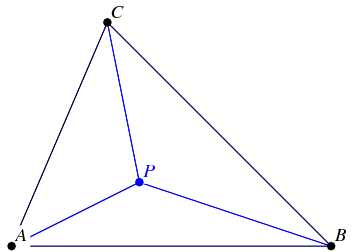
\includegraphics[scale=0.5]{img/triangulation.png}
\caption{The triangulation idea.}
\label{triangulation}
\end{center}
\end{figure}

Even with this solution we had lots of troubles about the precision of the localisation. It wasn't easy to determine with enough precision the position of a device close to the entering/exit doors and how much a user is close to each wall (maybe someone is trying to ``cheat" sticking the device close to a wall).
From this idea we thought that, since every room has four walls, the best idea was to triangulate the position using not three beacons but four of them.\\

\subsection{Our third implementation}
In this implementation we move closer to the implementation adopted by the Estimote's engineers: using four beacons, one for each wall of the room.\\

In fact we figured out that the increased a lot the localisation precision with this last implementation. By positioning a beacon in the center of each wall we could triangulate better the final position.\\

Even if we improved a lot the quality of the tracking there still were mainly two issues:
\begin{itemize}
\item In non-controlled environments, where you can find metals, and other objects that affect the signal, the received signal strength of the beacons changes so often that it seems impossible to get error range below 5 meters.
\item Depending on the way that the user is handling the receiver device, the readings can change a lot as well. If the user puts his/her hand over the bluetooth antenna, then the algorithm will have low signals as input, and thus the beacons will supposed to be very far from the device. See this image to see the precise location of the Bluetooth antenna.
\end{itemize}

\begin{figure}[htbp]
\begin{center}
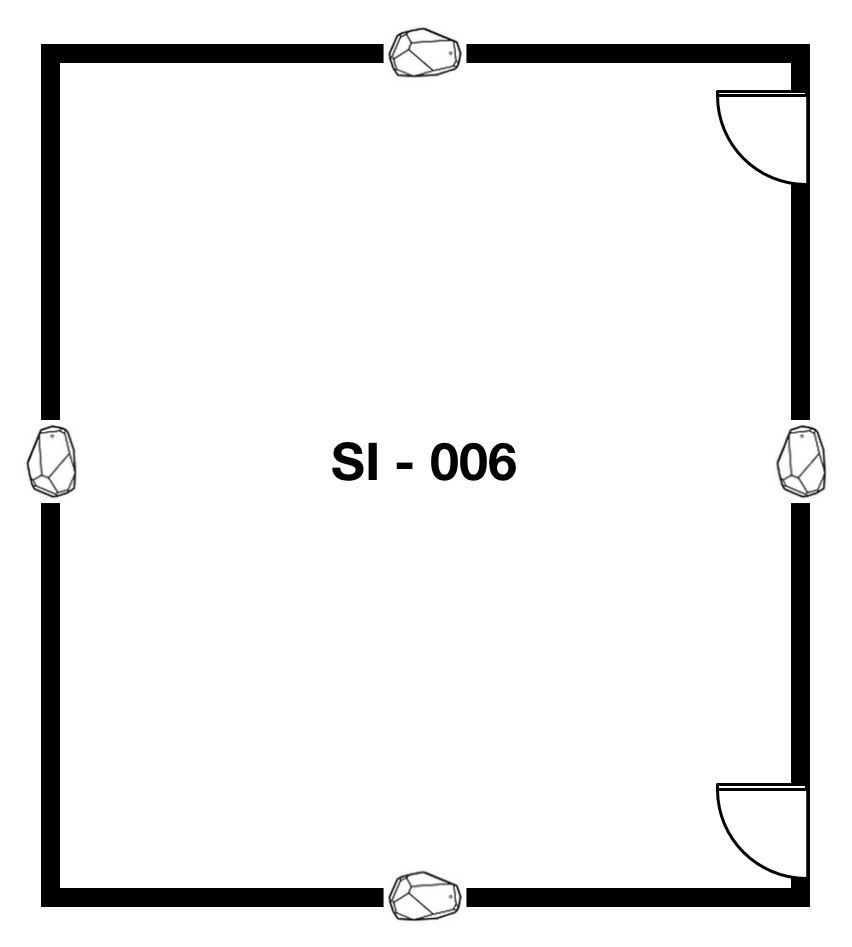
\includegraphics[scale=0.5]{img/room_beacon.png}
\caption{The final result with a triangulation done using three beacons.}
\label{room_beacon}
\end{center}
\end{figure}

\subsection{Our final implementation}
Since we moved closer and closer to the implementation adopted by Estimote we concluded that the best solution was to move to that implementation using the Estimote Frameworks (see \ref{estimoteframework}), available for free in the Estimote website. It uses the same idea we had in the third implementation but adds more then a year of refinement about error correction, wireless noise detection and reduction, as well as the possibility to map the position of each beacon respect to the others by counting the distance between them using an ad-hoc app developed by the Estimote.